\documentclass{article}
\usepackage[utf8]{inputenc}
\usepackage[hungarian]{babel}

\usepackage{lipsum}
\usepackage{graphicx}
\usepackage{titling}

\usepackage{fancyhdr}
\usepackage{pdfpages}


\begin{document}
	
	\begin{titlepage}
		\setlength{\headheight}{20pt}
		\lhead{
\includegraphics[height=1.5cm]{logo_mm.png}}
		\rhead{\Large{\textbf{Végeselem módszer alapjai}}\\
			BMEGEMMAGMV}
		%\vspace{15cm}
		\title{\huge Kötelező házi feladat 1
		}
		\author{Tar Dániel\\GUTOY7}
		\date{\today}
		\maketitle
		\pagenumbering{gobble}
		\thispagestyle{fancy}
		
		\begin{figure}
			\begin{center}
				
\includegraphics[height=2cm]{logo_bme_kicsi.eps}
			\end{center}
		\end{figure}
		
	\end{titlepage}
	\newpage

	%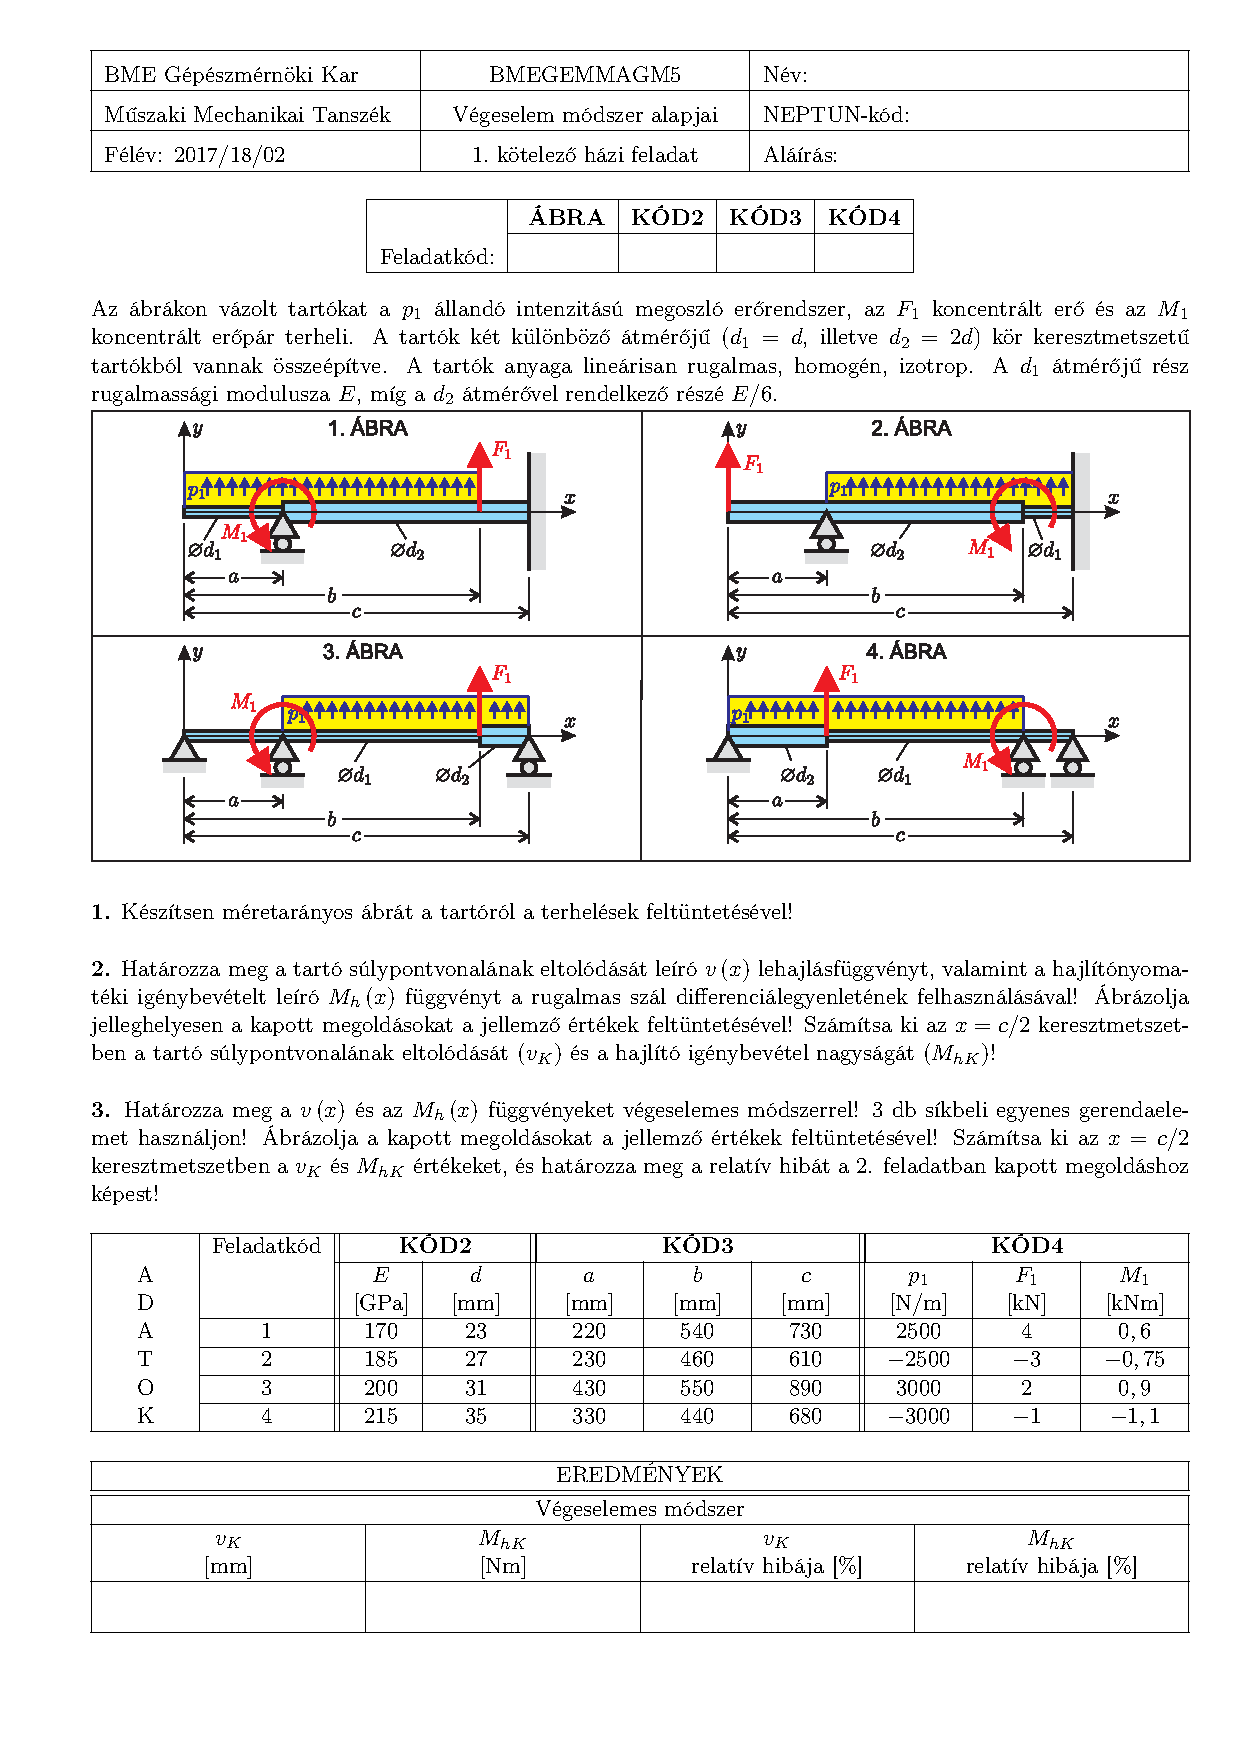
\includepdf{vemalaphf1.pdf}
	 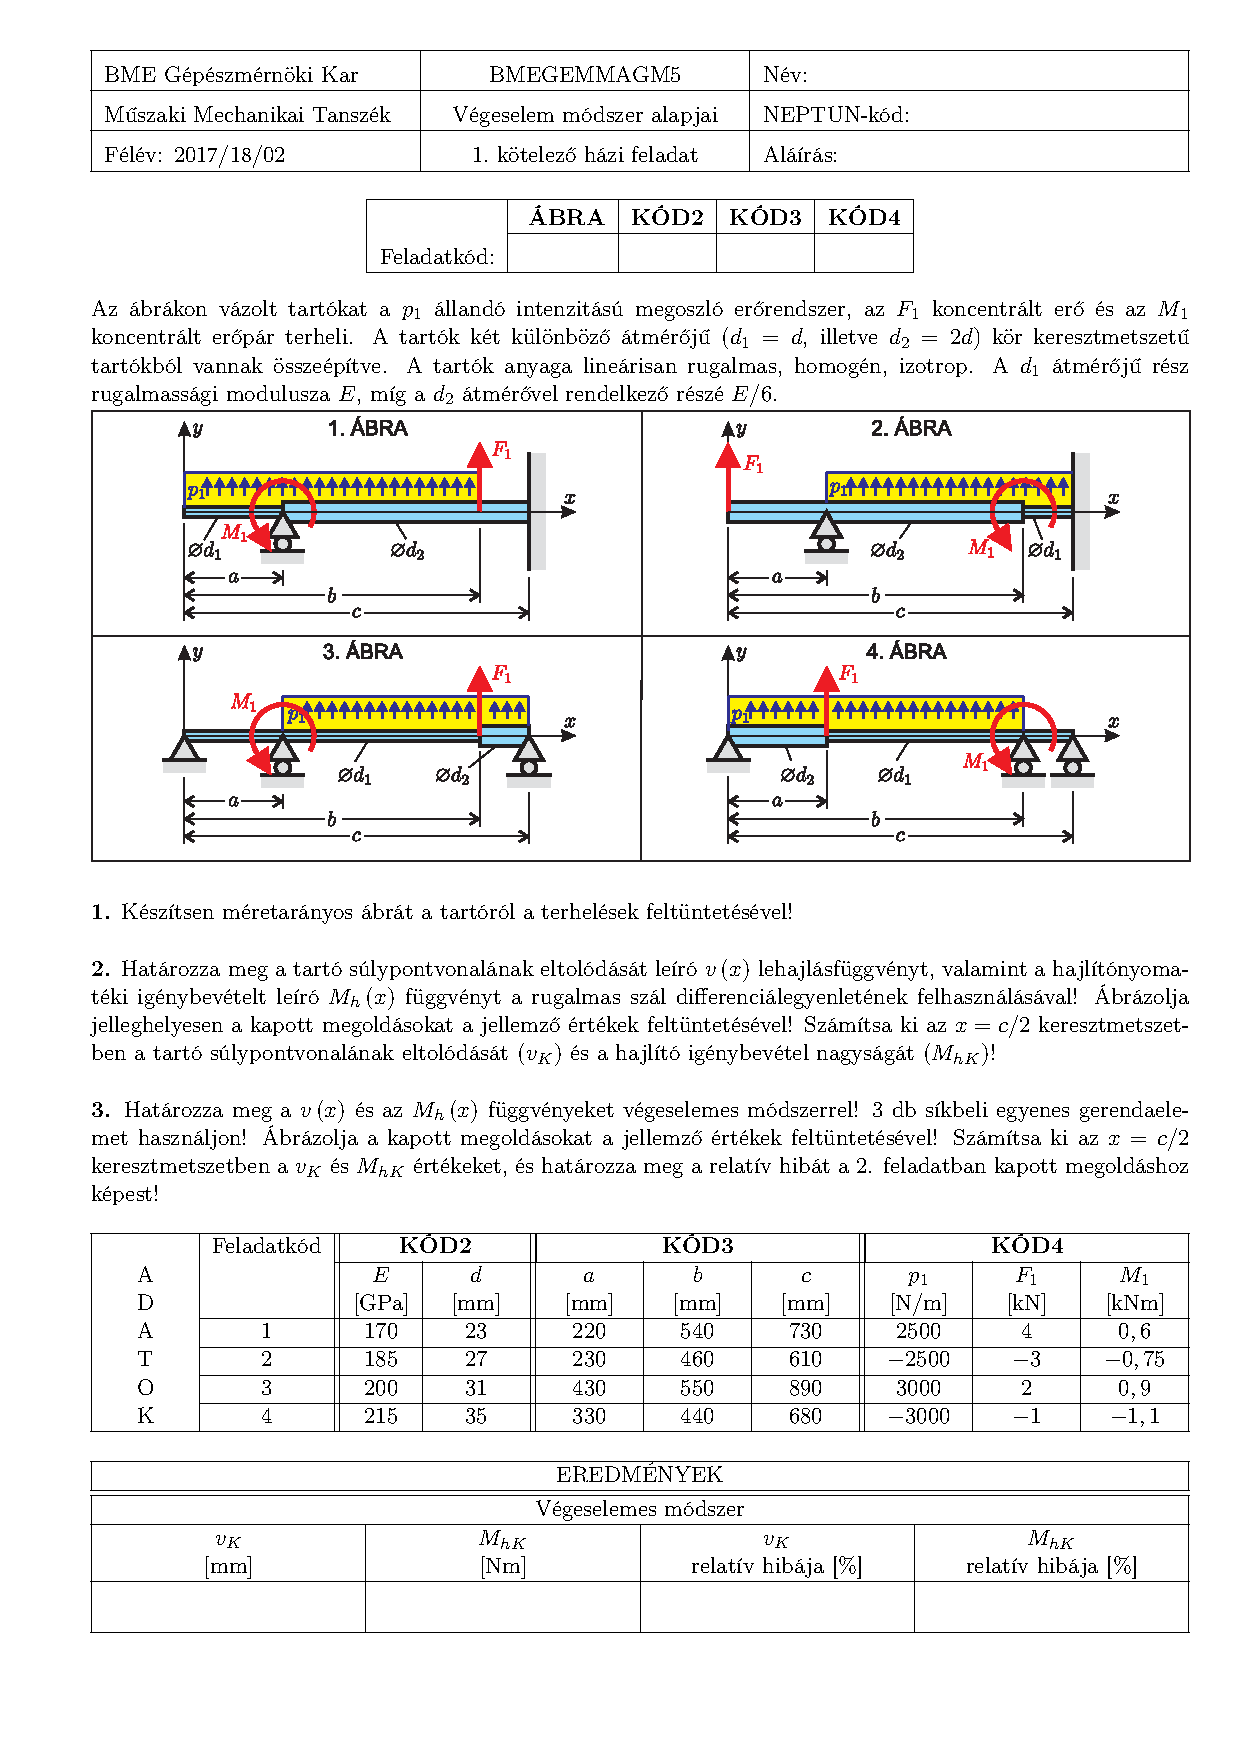
\includepdf[picturecommand*={
	    	\put(460,759){Tar Dániel}
	    	\put(460,740){GUTOY7}
	    	\put(280,677){2}
	    	\put(327,677){1}
	    	\put(370,677){2}
	    	\put(415,677){2}
	    	\put(115,63){eredmeny1}
	    	\put(245,63){eredmeny2}
	    	\put(370,63){eredmeny3}
	    	\put(490,63){eredmeny4}
	 }]{vemalaphf1.pdf}
	\newpage
	
	
	\setlength{\headheight}{0pt}
	\tableofcontents
	\newpage
	
	\pagenumbering{arabic}	
	\setcounter{page}{1}

	\section{Adatok}
	
		A házifeladat kód alapján az adatokat átszámolva $[N][mm][MPa]$ alapra:
	
	\begin{table}[h!]
		\begin{center}
			\caption{Adatok}
			\label{tab:table1}
			\begin{tabular}{c|c|c|c|c|c|c|c} % <-- Alignments: 1st column left, 2nd middle and 3rd right, with vertical lines in between
				$E$ & $d$ & $a$ & $b$ & $c$ & $p_{1}$ & $F_{1}$ & $M_{1}$ \\
				$[MPa]$ & $[mm]$ & $[mm]$ & $[mm]$ & $[mm]$ & $[N/mm]$ & $[N]$ & $[Nmm]$\\
				\hline
				$185\cdot10^3$ & 27 & 230 & 460 & 610 & -2.5 & -3000 & -0.75\\
				%2 & 10.1 & b\\
				%3 & 23.113231 & c\\
			\end{tabular}
		\end{center}
	\end{table}
	
	\begin{equation}
	f(x)=x^2
	\end{equation}
	
	\newpage
	
	\section{Feladat}
	
	
	
	This formula $f(x) = x^2$ is an example.

\end{document}
